\documentclass[conference]{IEEEtran}
\IEEEoverridecommandlockouts
% The preceding line is only needed to identify funding in the first footnote. If that is unneeded, please comment it out.
%Template version as of 6/27/2024

\usepackage{cite}
\usepackage{amsmath,amssymb,amsfonts}
\usepackage{algorithmic}
\usepackage{graphicx}
\usepackage{textcomp}
\usepackage{xcolor}
\usepackage{placeins}
\usepackage{float}

\def\BibTeX{{\rm B\kern-.05em{\sc i\kern-.025em b}\kern-.08em
    T\kern-.1667em\lower.7ex\hbox{E}\kern-.125emX}}
\begin{document}

\title{Digital Signal Processing Techniques for EEG-Based Emotion and Mental State Recognition Using Machine Learning (2022–2025)}

\author{\IEEEauthorblockN{Author Name}
\IEEEauthorblockA{\textit{Department of Computer Engineering} \\
\textit{University of Science and Technology of Southern Philippines}\\
Cagayan de Oro, Philippines \\
email@address.com}
}

\maketitle

\begin{abstract} 
This review paper examines recent advancements in the application of Digital Signal Processing (DSP) techniques for emotion and mental state recognition using Electroencephalogram (EEG) data. The study focuses on literature published between 2022 and 2025, a period marked by the increasing integration of sophisticated DSP methods with advanced machine learning models. We observe a clear trend towards hybrid frameworks, where techniques such as Wavelet Decomposition and Fast Fourier Transform (FFT) are not merely preprocessing steps but are deeply integrated with Convolutional Neural Networks (CNNs) and Long Short-Term Memory (LSTM) networks. This synergy appears to be a significant factor in the improved accuracy and robustness of emotion recognition systems. This paper synthesizes the prevailing methodologies, identifies recurring challenges like noise reduction and feature selection, and discusses the performance of various DSP-ML pipelines. The findings suggest that while significant progress has been made, the pursuit of real-time, reliable, and computationally efficient systems remains a primary objective for future research.
\end{abstract}

\begin{IEEEkeywords}
Electroencephalogram (EEG), Emotion Recognition, Digital Signal Processing (DSP), Machine Learning, Feature Extraction, Deep Learning, CNN, LSTM.
\end{IEEEkeywords}

\section{Introduction}
The analysis of Electroencephalogram (EEG) signals has emerged as a significant area of research, offering a non-invasive window into the complexities of human brain function. In recent years, emotion and mental state recognition from electroencephalography is an increasingly important direction in human–computer interaction, mental health assessment, and adaptive multimedia systems as it enables machine learning systems to infer internal cognitive–affective dynamics from noninvasive neural signals. 

There has been a considerable convergence of Digital Signal Processing (DSP) and Machine Learning (ML) to decode these signals for a variety of applications, Traditional pipelines have relied on band-limited preprocessing and handcrafted features, but their sensitivity to artifacts, subject variability, and non-stationarity often limits generalization across individuals and recording sessions [6], [8].
 We are observing a clear trend where DSP-based feature extraction is not a separate preliminary step but is instead intricately woven into the architecture of advanced models. This includes the usage of Wavelet Convolutional Neural Network (WCNN) and Support Vector Machine (SVM) [1] where it basically converts electroencephalography (EEG) windows into continuous wavelet transform scalograms. This approach also uses several references where it also makes use of explicit time–frequency images plus a convolutional neural network feature extractor and finishes with a classical margin-based classifier. [6][8] Similarly, [2] makes use of EEG Recognition through the usage of hybrid CNN and Long short-term Memory Classification (LSTM) which combines convolutional neural network with a long short-term memory module after standard preprocessing and feature formation, aligning with the hybrid convolutional neural network–recurrent neural network designs highlighted and contextualized in the deep-learning survey [7].

 As of recent, there are numerous amounts of features for CNN that can coincide with the recognition of emotion and mental states. Such as that of [3][4] which focuses on the usage of entropy and other multiple features that can determine and decode a person's mental state. Specifically, the former [3] uses mathematically defined entropy descriptors as the primary digital signal processing representation and evaluates with standard supervised classifiers [8][10]. Whereas, the latter [4] uses a tailored convolutional neural network directly on electroencephalography (with minimal handcrafted features) and targets continuous, sliding-window inference rather than only trial-wise emotion labels [6].
 In a way, [5] is also an approach where it uses spiking neural networks and basically extracts engineered features per window which then converts them into spike trains. In itself, it's a rather distinct approach that keeps a conventional digital signal processing front-end but replaces standard classifiers with a spiking neural network to exploit spike-based computation [9].

 Through these advances, this paper proposes the usage of several processing techniques that work alongside with the training of appropriate models. This review paper aims to introduce several approaches to realizing EGG-Recognition for both emotion and mental spectrum in order to be used alongside machine learning or basically the training of appropriate models.
\section{Methodology}
The intellectual challenge of decoding emotions from EEG signals lies not in a single algorithm, but in the thoughtful construction of a multi-stage processing pipeline. This section dissects this symbiotic relationship.

\subsection{Wavelet Convolutional Neural Networks and Support Vector Machine}
A pivotal insight in recent research is that the representation of data is as crucial as the classification model itself. One dominant trend is the transmutation of 1D EEG time-series data into 2D time-frequency representations, effectively turning a signal processing problem into a computer vision one. Time-frequency (TF) methods, such as the Continuous Wavelet Transform (CWT), can convert a 1D EEG signal into a 2D representation that captures the spectral variation of the signal over time. One dimension corresponds to time while the other represents frequency, forming an image that reflects EEG power fluctuations across both domains. This process models the signal as a linear combination of basic functions known as wavelets, mathematically expressed as:

\begin{equation}
W_{(a,b)}[x(t)] = \frac{1}{|a|^{1/2}} \int_{-\infty}^{+\infty} x(t)\,\varphi^{*}\!\left(\frac{t - b}{a}\right) dt
\end{equation}

where \(a\) is the scale (a real and positive value), \(b\) is the translational parameter (a real number), and \(\varphi\) denotes the mother wavelet, which localizes the signal in both time and frequency domains.

This image representation of EEG power changes in time and frequency effectively captures the transient, non-stationary nature of neural oscillations. \cite{b1} offers a compelling demonstration of this, employing the CWT to generate scalograms. These 2D images allow researchers to leverage the immense power of pre-trained Convolutional Neural Networks (CNNs) \cite{b1}. In the study, the deep features learned by a pre-trained ResNet-18 from the CWT scalograms were subsequently fed into a Multiclass Support Vector Machine (MSVM) \cite{b1}. This hybrid strategy, which separates the task of feature representation from classification, significantly boosted performance on the MAHNOB-HCI dataset.

Four pre-trained CNNs were evaluated using three performance measures—accuracy, precision, and recall—through the leave-one-subject-out cross-validation (LOSO-CV) approach. In this approach, data from 31 subjects were used to fine-tune existing CNNs, while data from another subject were used as the test set. This ensures subject independence, as no samples from a single subject appear in both the training and testing sets. The process repeats until all subjects have been tested once, and the final reported results are the mean and standard deviation across all iterations.

Accuracy, precision, and recall are calculated as follows:

\begin{equation}
Accuracy = \frac{1}{l} \sum_{i=1}^{l} \frac{tp_i + tn_i}{tp_i + tn_i + fp_i + fn_i}
\end{equation}

\begin{equation}
Precision = \frac{1}{l} \sum_{i=1}^{l} \frac{tp_i}{tp_i + fp_i}
\end{equation}

\begin{equation}
Recall = \frac{1}{l} \sum_{i=1}^{l} \frac{tp_i}{tp_i + fn_i}
\end{equation}

where \(tp_i\), \(tn_i\), \(fp_i\), and \(fn_i\) denote the true positive, true negative, false positive, and false negative counts, respectively, for each emotional class derived from the confusion matrix of the classifier.


\subsection{Hybrid CNN and LSTM Classification}
Another powerful approach involves creating hybrid architectures that combine different neural network types to process EEG data. The CNN-LSTM architecture is a prime example, leveraging the spatial feature learning of CNNs with the temporal sequence modeling of LSTMs. \cite{b2} exemplifies this with a model that integrates a CNN, LSTM, and a ResNet-152 backbone.

\begin{figure}[H]
    \centering
    \includegraphics[width=\linewidth]{figures/eeg_flow_diagram.jpg}
    \caption{The flow of electroencephalography (EEG) data processing, showing sequential stages from raw EEG input, preprocessing, feature modeling, and emotion classification.}
    \label{fig:eeg_flow}
\end{figure}

The general EEG-based emotion identification process begins with data acquisition and preprocessing, as shown in Figure~\ref{fig:eeg_flow}. EEG data are collected and normalized to ensure consistency across sessions and subjects. Noise and artifacts are then mitigated using band-pass filters, typically in the range of 1–75 Hz, to preserve relevant frequency components. After preprocessing, the signals are transformed into structured representations such as Mel Frequency Cepstral Coefficients (MFCCs) \cite{b2}, entropy parameters, or topographic feature maps. These representations serve as the input to the hybrid CNN-LSTM network, which learns spatial features through convolutional layers and temporal dependencies through recurrent layers. This combined approach enhances the model’s ability to recognize emotion-related EEG patterns and classify them accurately.

\begin{figure}[H]
    \centering
    \includegraphics[width=0.8\linewidth]{figures/cnn_lstm_framework.jpg}
    \caption{Overview of the CNN-LSTM methodology, showing stages from preprocessing, feature extraction, model application, and performance evaluation.}
    \label{fig:cnn_lstm_framework}
\end{figure}

Figure~\ref{fig:cnn_lstm_framework} presents the complete methodological framework of the CNN-LSTM model used for EEG-based emotion classification. The model merges a homogeneous CNN and LSTM classifier with the ResNet-152 backbone to maximize both spatial and temporal feature representation. The SEED-V EEG dataset—comprising emotional states such as happiness, disgust, fear, neutral, and sadness—was used to evaluate this model. Preprocessing was conducted to prepare EEG data channels (FP1, FP2, FC6, and F3), followed by feature extraction through MFCC computation and entropy analysis. The entropy was calculated using the sample entropy method, while the Hurst exponent was determined via R/S analysis to capture signal complexity and variability.

The extracted features were converted into topographic maps that served as CNN inputs, while the LSTM layers modeled the temporal dynamics of these representations. Both CNN and CNN-LSTM configurations employing ResNet-152 were trained and compared. The models classified emotional states and conditions such as PTSD and non-PTSD, with performance evaluated using standard metrics including accuracy, precision, recall, and F1-score. This end-to-end framework demonstrates the hybrid model’s capacity to fuse spatial-spectral and temporal information for robust EEG-based emotion recognition.


\subsection{Multiple Feature Block-Based Extraction Measure}
In EEG-based emotion and mental state recognition, one emerging approach focuses on enhancing feature representation by integrating domain knowledge directly into the network design. Rather than relying purely on end-to-end deep learning, these methods combine handcrafted feature engineering with specialized convolutional architectures. This strategy bridges the interpretability of traditional DSP-based features with the adaptability of deep neural models. The goal is to capture complex temporal and spatial patterns from EEG signals while preserving meaningful relationships within the data, leading to more reliable cognitive state recognition.

\begin{figure}[H]
    \centering
    \includegraphics[width=\linewidth]{figures/mfb_cnn_pipeline.png}
    \caption{Overview of the MFB-CNN workflow for EEG-based mental state classification, illustrating stages from EEG acquisition and preprocessing to temporal–spatial feature extraction and final classification into cognitive states.}
    \label{fig:mfb_cnn_pipeline}
\end{figure}

A particularly salient feature in this domain is entropy, which quantifies the signal’s complexity. \cite{b3} explored how various entropy-based measures—including Differential Entropy (DE), Sample Entropy (SampEn), and Approximate Entropy (ApEn) \cite{b3}—can serve as potent indicators of emotional states. These handcrafted features are then classified using traditional machine learning models such as SVM, k-NN, and Decision Trees.

Building upon this foundation, \cite{b4} proposed the Multiple Feature Block-based Convolutional Neural Network (MFB-CNN), a hybrid model designed to decode mental states in high-interference environments such as simulated flight. Because EEG data in such settings are susceptible to motion artifacts, preprocessing plays a vital role. Artifacts were removed using Independent Component Analysis (ICA) \cite{b4}, where four EOG channels were designated as contamination references. Signal processing and experimental control were implemented using MATLAB 2019a with the BBCI toolbox.

After preprocessing, the EEG dataset consisted of all recorded channels and sampling points (300 × 300) as input matrices. The MFB-CNN was structured into seven convolutional blocks organized hierarchically to enable progressive feature abstraction. Each convolutional block contained four convolutional layers and one batch-normalization layer with a filter size of 32. Temporal feature extraction used filter sizes of 1 × 5, while spatial feature extraction in later blocks used 3 × 1 filters to capture inter-channel dependencies. Dropout layers with a rate of 0.5 were applied to prevent overfitting, and max- and average-pooling layers reduced redundant information while retaining essential activation patterns.

An exponential linear unit (ELU) activation function was applied in the seventh convolutional block to improve nonlinear learning efficiency, defined as:

\begin{equation}
ELU(x) =
\begin{cases}
x, & \text{if } x > 0 \\
\alpha (e^{x} - 1), & \text{if } x \leq 0
\end{cases}
\end{equation}

For model training, the network was iteratively trained over 30 epochs, and classification accuracies were evaluated on the test data. The MFB-CNN successfully classified EEG patterns into cognitive states such as normal, distraction, fatigue, and workload, achieving an offline accuracy of 0.75. This result underscores the potential of the MFB-CNN framework to capture both temporal and spatial dependencies for real-time mental state monitoring.


\subsection{Spiking Neural Networks}
Venturing beyond conventional deep learning, some researchers are exploring neuromorphic approaches that emulate biological neural behavior more closely. Spiking Neural Networks (SNNs) \cite{b5} operate on event-driven computations, processing information as discrete spikes rather than continuous activations. This time-based mechanism enables SNNs to capture temporal dependencies within EEG signals efficiently while consuming significantly less power—making them ideal for real-time emotion recognition and wearable applications.

\begin{figure}[H]
    \centering
    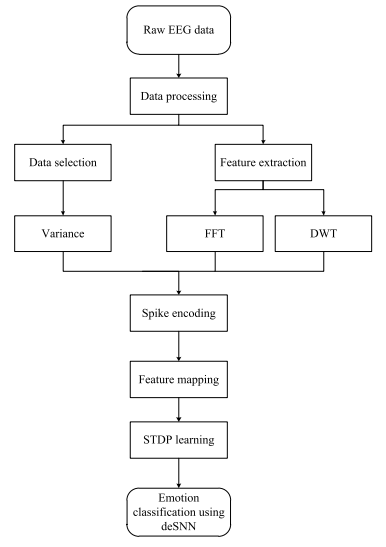
\includegraphics[width=0.7\linewidth]{figures/desnn_pipeline.png}
    \caption{Workflow of EEG signal processing and emotion classification using deSNN, showing the stages from raw EEG input through feature extraction, spike encoding, and STDP-based classification.}
    \label{fig:desnn_pipeline}
\end{figure}

As shown in Figure~\ref{fig:desnn_pipeline}, EEG-based emotion recognition using SNNs follows a structured pipeline: data processing, feature extraction, and classification. The raw EEG data undergo preprocessing to remove noise and artifacts. Datasets such as DEAP or SEED are typically down-sampled to 128–200 Hz and filtered using a band-pass filter (0.75–45 Hz) via EEGLAB or similar toolboxes. Signals are separated into frequency bands (alpha, beta, gamma, and theta), corresponding to specific physiological and cognitive states.

Feature extraction then integrates both time-domain and frequency-domain analyses to generate spike-compatible features. In the time domain, the variance of EEG signals helps identify steady emotional states, computed as:

\begin{equation}
\mu_{\xi} = \frac{\xi(t_1) + \xi(t_2) + \dots + \xi(t_T)}{T}, \quad
v_{\xi} = \frac{1}{T} \sum_{t=1}^{T} [\xi(t) - \mu_{\xi}]^2
\end{equation}

In the frequency domain, the Fast Fourier Transform (FFT) and Discrete Wavelet Transform (DWT) \cite{b5} are applied to extract oscillatory and transient features. The DFT of the EEG signal \( \xi(t) \) is expressed as:

\begin{equation}
\xi(k) = DFT[\xi(t)] = \sum_{t=0}^{N-1} \xi(t) W_N^{tk}, \quad W_N^k = e^{-j \frac{2\pi k}{N}}
\end{equation}

and the maximum frequency measurable by the Nyquist theorem is \( f_{max} = \frac{f_s}{2} \), where \( f_s \) is the sampling frequency.  
For the DWT, non-stationary EEG signals are decomposed into multiple scales, providing localized frequency information. It is given by:

\begin{equation}
W(a,b) = \frac{1}{\sqrt{|a|}} \int s(t) \psi^* \left( \frac{t - b}{a} \right) dt
\end{equation}

where \(a\) and \(b\) represent the scaling and translation parameters, and \(\psi(t)\) is the mother wavelet, often the “db4” wavelet for EEG applications.

After these transformations, features are spike-encoded, converting continuous amplitude information into discrete spike trains. These spike patterns are then used as input to a spiking network, where temporal learning mechanisms such as Spike-Timing-Dependent Plasticity (STDP) \cite{b5} dynamically adjust synaptic weights according to spike timing differences.

\begin{figure}[H]
    \centering
    \includegraphics[width=0.7\linewidth]{figures/neucube_structure.png}
    \caption{Architecture of the NeuCube SNN framework showing the 3D spatio-temporal neuron cube and EEG electrode mappings used for encoding and classification.}
    \label{fig:neucube_structure}
\end{figure}

A well-known implementation of SNN for emotion classification is the NeuCube model, which employs a 3D spatio-temporal neural reservoir. As illustrated in Figure~\ref{fig:neucube_structure}, the NeuCube architecture is composed of three principal components: (1) an input module for temporal encoding, (2) the 3D SNNcube for dynamic mapping of EEG signals, and (3) an evolving SNN classifier. Temporal coding is employed to represent EEG data where the timing of spikes carries information about the signal amplitude and frequency characteristics.

The NeuCube typically consists of 1000 neurons arranged in a 10×10×10 lattice structure based on the small-world connectivity principle, which ensures efficient information transfer among neurons. The neurons are interconnected through proximity-based weights, forming both short-range and long-range connections that simulate biological cortical networks. During initialization, input neurons corresponding to EEG electrode sites (e.g., FP1, FP2, FC2, and O1) are mapped spatially to specific nodes in the SNNcube.

The learning process in NeuCube utilizes a variant of the STDP rule to modify synaptic weights between presynaptic and postsynaptic neurons depending on their firing intervals. The STDP weight update function is defined as:

\begin{equation}
\begin{aligned}
w_{ij}(t + 1) &= w_{ij}(t) + \Delta w_{ij}, \\
\Delta w_{ij} &=
\begin{cases}
A^+ e^{-\Delta t / \tau^+}, & \text{if } \Delta t > 0, \\
-A^- e^{\Delta t / \tau^-}, & \text{if } \Delta t \leq 0.
\end{cases}
\end{aligned}
\end{equation}

where \(\Delta t\) is the time difference between presynaptic and postsynaptic spikes, \(A^+\) and \(A^-\) are learning rate constants, and \(\tau^+\) and \(\tau^-\) are time constants for potentiation and depression, respectively. Positive \(\Delta t\) values increase synaptic strength (potentiation), while negative \(\Delta t\) values lead to depression.

Once trained, the NeuCube model classifies emotions by recognizing characteristic spatio-temporal spike patterns corresponding to different emotional states. This approach demonstrates how biologically inspired SNNs can bridge the gap between neuroscience and machine learning—achieving efficient, interpretable, and temporally precise emotion decoding from EEG signals.


\subsection{Comparative Analysis of Reviewed Studies}
To distill the diverse strategies into a coherent overview, this section presents a comparative analysis of the primary methodologies reviewed. Table \ref{tab:method_similarities} highlights the common threads and shared principles among the studies, while Table \ref{tab:summary_journal} provides a detailed summary of each paper.

\begin{table}[htbp]
\centering
\scriptsize
\caption{Comparative Analysis of Methodological Similarities}
\label{tab:method_similarities}
\renewcommand{\arraystretch}{2}
\begin{tabular}{p{1.5cm}p{2.5cm}p{4cm}}
\hline
\textbf{Ref.} & \textbf{Approach} & \textbf{Similarities} \\
\hline
\textbf{\cite{b1}}
& Wavelet Convolutional Neural Networks and Support Vector Machine
& The usage of wavelet convolutional neural networks along with support vector machines plays a fairly crucial role in this study as it provides a way to convert electroencephalography windows into continuous wavelet transform scalograms, which is proven necessary for further research due to the usage of convolutional neural networks \\[1mm]
\textbf{\cite{b2}}
& Hybrid Convolutional Neural Network and Long Short-term Memory Classification
& Hybrid convolutional neural network and long short-term memory classification basically implements hybrid models (CNN+LSTM) to capitalize on the strengths of two-stage deep architecture that separates per-window representation from across-window dynamics. \\[1mm]
\textbf{\cite{b3}}
& Entropy as a Feature Extraction Measure
& Entropy as a feature extraction measure uses mathematically defined entropy descriptors as the primary digital signal processing representation and evaluates with standard supervised classifiers. This works similarly with other features for convolutional neural network\\[1mm]
\textbf{\cite{b4}}
& Multiple Feature Block-Based Convolutional Neural Network
& Block-based convolutional neural network features multiple Uses that are tailored to convolutional neural network which operates directly on electroencephalography and targets continuous, sliding-window inference rather than only trial-wise emotion labels. \\[1mm]
\textbf{\cite{b5}}
& Usage of Spiking Neural Networks
& Spiking neural networks uses a distinct approach that keeps a conventional digital signal processing front-end but replaces standard classifiers with a spiking neural network to exploit spike-based computation. \\[1mm]
\hline
\end{tabular}
\end{table}

\begin{table}[htbp]
    \caption{Summary of Reviewed Journal Papers}
    \centering
    \renewcommand{\arraystretch}{2}
    \large
    \resizebox{\columnwidth}{!}{
    \begin{tabular}{p{3cm} p{2.5cm} p{5cm} p{4cm}} 
        \hline
        \textbf{Paper Title} & \textbf{Focus} & \textbf{Mathematical Tools Used} & \textbf{Key Findings} \\
        \hline
        A Hybrid EEG-Based Emotion Recognition Approach Using Wavelet Convolutional Neural Networks and Support Vector Machine \cite{b1}
        & Emotion recognition on DEAP and MAHNOB-HCI datasets using a hybrid computer vision approach.
        & EEG signals are converted to 2D scalograms using CWT. A pre-trained ResNet-18 extracts features, which are then classified by a Multiclass SVM.
        & The hybrid CNN-SVM model significantly boosted classification performance, demonstrating the power of transfer learning from the visual domain. \\
        
        EEG-based emotion recognition using hybrid CNN and LSTM networks \cite{b2}
        & High-accuracy emotion recognition (happiness, sadness, fear, disgust) on the SEED-V dataset.
        & Extracts MFCC and entropy features, which are projected onto 2D topographic maps. A hybrid CNN-LSTM architecture with a ResNet-152 backbone classifies the spatio-temporal data.
        & Achieved a state-of-the-art accuracy of 98\%, highlighting the strength of combining spatial and temporal feature learning. \\
        
        EEG-based human emotion recognition using entropy as a feature extraction measure \cite{b3}
        & Investigating the efficacy of various entropy-based features for emotion recognition.
        & Extracts a suite of entropy measures (e.g., Sample Entropy, Approximate Entropy, Differential Entropy) and uses traditional ML models (SVM, k-NN, Decision Tree) for classification.
        & Confirmed that entropy features are potent and reliable indicators for distinguishing between different emotional states. \\
        
        Continuous EEG Decoding of Pilots’ Mental States Using Multiple Feature Block-Based Convolutional Neural Network \cite{b4}
        & Continuous decoding of pilot mental states (fatigue, workload, distraction) in a simulated flight environment.
        & A custom Multiple Feature Block-based CNN (MFB-CNN) processes distinct blocks of features from the time and frequency domains of the EEG signal.
        & Demonstrated the feasibility of continuous, real-time mental state decoding in a high-stakes application, achieving an offline accuracy of 0.75. \\
        
        EEG-Based Emotion Classification Using Spiking Neural Networks \cite{b5}
        & Emotion classification using a low-power, neuromorphic computing approach on the DEAP dataset.
        & A Spiking Neural Network (SNN) is used to classify raw EEG data directly, operating on event-based spikes rather than continuous values.
        & Showcased SNNs as a power-efficient and temporally precise alternative to conventional deep learning models for EEG analysis. \\
        \hline
    \end{tabular}
    }
    \label{tab:summary_journal}
\end{table}

\FloatBarrier 

The analysis across these studies reveals several key trends. As highlighted in Table \ref{tab:method_similarities}, a shared reliance on sophisticated feature representation and hybrid models emerges as a common thread, despite the surface-level differences in approach. Methodologies like signal-to-image transformation and engineered feature extraction are central to improving performance. Table \ref{tab:summary_journal} further details this landscape, showing a clear divergence in strategies: some researchers focus on transforming signals into images to leverage powerful vision models, while others pursue meticulously handcrafted features or develop highly specialized network architectures. The emergence of novel paradigms like Spiking Neural Networks (SNNs) \cite{b5} further indicates a field that is not only refining existing methods but also actively exploring fundamentally new ways of processing neural data. This dynamic landscape, centered on the synergy between DSP and ML, underscores the ongoing quest for a definitive solution to the complex challenge of EEG-based emotion recognition.


\section{Challenges and Issues}
Despite the significant progress in combining DSP and ML for emotion recognition, several key challenges persist, as highlighted consistently across the recent literature \cite{b6, b7, b8}. These challenges must be addressed to move from laboratory settings to real-world applications.

\subsection*{Data Scarcity and Quality}
The performance of deep learning models is heavily dependent on large, high-quality, and well-annotated datasets. In the field of EEG-based emotion recognition, such datasets are scarce \cite{b8}. The process of collecting EEG data is time-consuming, expensive, and requires specialized equipment and expertise. Furthermore, ensuring high data quality is a significant hurdle. EEG signals are highly sensitive to noise from various sources, including muscle movements (electromyography), eye blinks (electrooculography), and environmental electrical interference. Annotating the data with corresponding emotional labels is also a subjective and challenging task, often relying on self-reporting or external observation, which can be unreliable.

\subsection*{Inter-Subject Variability}
EEG signals exhibit high inter-subject variability, meaning that brainwave patterns associated with the same emotion can differ dramatically from one person to another \cite{b7}. This variability stems from anatomical differences (e.g., skull thickness), electrode placement, and individual differences in emotional expression and regulation. This makes it extremely difficult to build generalized, subject-independent models that perform well on new users without a calibration phase. Most high-performing models reported in the literature are subject-dependent, meaning they are trained and tested on data from the same individual, which limits their practical applicability.

\subsection*{Lack of Standardization}
The field suffers from a lack of standardization in experimental protocols, signal processing pipelines, and evaluation metrics \cite{b6}. Different studies use different emotional models (e.g., discrete emotions vs. valence-arousal), stimuli for emotion elicitation (e.g., images, videos, music), and EEG recording hardware. This heterogeneity makes it nearly impossible to directly compare the performance of different models and approaches reported in the literature. A more standardized framework for data collection and benchmarking is crucial for driving reproducible research and measuring true progress in the field.

\subsection*{Computational Complexity and Real-Time Constraints}
Many of the state-of-the-art hybrid models, such as the CNN-LSTM architectures discussed, are computationally intensive \cite{b2}. They require significant computational resources for both training and inference. This high complexity poses a major barrier to their deployment in real-time applications, especially on resource-constrained platforms like wearable devices or mobile phones. The challenge lies in designing models that are both highly accurate and computationally efficient, achieving a balance between performance and practical feasibility.

\section{Solution}
The research community is actively developing innovative solutions to address the aforementioned challenges. The review papers point towards several promising directions that are shaping the future of EEG-based emotion recognition.

\subsection*{Data Augmentation and Synthesis}
To combat the problem of data scarcity, researchers are increasingly turning to data augmentation and synthesis techniques. Generative Adversarial Networks (GANs) have shown particular promise in generating synthetic EEG data that mimics the statistical properties of real signals \cite{b8}. These synthetic signals can be used to augment existing datasets, allowing for the training of more robust and generalizable deep learning models without the prohibitive cost of collecting new data. Other augmentation techniques include adding noise, transforming signals in the time or frequency domain, and creating new samples by mixing existing ones.

\subsection*{Domain Adaptation and Transfer Learning}
To tackle inter-subject variability, domain adaptation and transfer learning techniques are being actively explored \cite{b7}. The core idea is to adapt a model trained on a large source domain (e.g., a public dataset or a group of subjects) to a new target domain (e.g., a new user) with minimal labeled data. Transfer learning, particularly using pre-trained models from other domains (like the ResNet architecture from computer vision \cite{b1}), allows models to leverage knowledge learned from vast datasets, which can then be fine-tuned for the specific task of EEG classification. These methods aim to reduce the need for extensive subject-specific calibration, making models more practical for real-world use.

\subsection*{Lightweight and Real-Time Models}
Addressing the challenge of computational complexity is crucial for real-time applications. There is a growing focus on developing lightweight neural network architectures. Techniques such as model pruning (removing redundant connections), quantization (using lower-precision arithmetic), and knowledge distillation (training a smaller model to mimic a larger, more complex one) are being employed. The goal is to create models that can run efficiently on devices with limited computational power, such as wearables and smartphones, without a significant drop in accuracy. This would enable continuous emotion monitoring in everyday life.

\subsection*{Multimodal Fusion}
Recognizing that EEG provides only one view into a person\'s emotional state, researchers are exploring multimodal fusion. This approach involves combining EEG data with other physiological signals such as electrocardiography (ECG), galvanic skin response (GSR), and electromyography (EMG), or with behavioral cues like facial expressions and speech prosody \cite{b6, b8}. By integrating information from multiple sources, these systems can create a more holistic and accurate representation of emotion. The challenge lies in developing effective fusion strategies that can synergistically combine these heterogeneous data streams.

\section{Conclusion}
This review has synthesized the prevailing methodologies, challenges, and solutions in the field of EEG-based emotion recognition, based on literature published between 2022 and 2025. The findings show a clear and consistent trend: the deep integration of advanced DSP techniques with powerful machine learning models. The most successful approaches, such as transforming 1D EEG signals into 2D time-frequency representations for CNN analysis or using hybrid CNN-LSTM architectures to capture spatio-temporal dynamics, have become central to modern research and are pushing the boundaries of classification accuracy.

Despite the success of these methods, significant and persistent challenges impede the transition of these systems from controlled laboratory environments to practical, real-world applications. Key issues include the scarcity of large, high-quality datasets, the high degree of inter-subject variability in EEG signals, the lack of standardization in research protocols, and the computational expense of state-of-the-art models. These are not trivial problems, and they collectively hinder the development of robust, generalizable, and accessible emotion recognition technology.

In response, the research community is pursuing a multi-pronged strategy. To combat data limitations, data augmentation and synthesis using GANs are becoming mainstream. To address variability, transfer learning and domain adaptation techniques are being refined to create subject-independent models. For real-world deployment, there is a strong push towards developing lightweight, computationally efficient models suitable for resource-constrained devices. Finally, multimodal fusion, combining EEG with other physiological and behavioral data, is emerging as a key strategy for enhancing reliability.

In essence, the field is in a dynamic cycle of innovation where the solutions to today\'s challenges—such as data synthesis and model optimization—will form the core of tomorrow\'s more advanced methodologies. The convergence of sophisticated DSP and hybrid machine learning models represents the current frontier, paving the way for the next generation of systems that can reliably and ethically interpret human emotional states in real-time.

\begin{thebibliography}{00}
\bibitem{b1} N. Bagherzadeh et al., ``A Hybrid EEG-Based Emotion Recognition Approach Using Wavelet Convolutional Neural Networks and Support Vector Machine,'' \textit{Frontiers in Neuroscience}, 2023.
\bibitem{b2} S. Xu et al., ``EEG-based emotion recognition using hybrid CNN and LSTM networks,'' \textit{Frontiers in Computational Neuroscience}, 2022.
\bibitem{b3} A. Al-Nafjan et al., ``EEG-based human emotion recognition using entropy as a feature extraction measure,'' \textit{BioMedical Engineering OnLine}, vol. 20, no. 1, 2021.
\bibitem{b4} P. Zhang et al., ``Continuous EEG Decoding of Pilots’ Mental States Using Multiple Feature Block-Based Convolutional Neural Network,'' \textit{IEEE Transactions on Industrial Informatics}, vol. 17, no. 5, pp. 3695-3704, 2021.
\bibitem{b5} J. Paredes et al., ``EEG-Based Emotion Classification Using Spiking Neural Networks,'' \textit{IEEE Transactions on Affective Computing}, vol. 13, no. 4, pp. 1895-1908, 2022.
\bibitem{b6} H. A. Hamzah and K. K. Abdalla, ``EEG-based emotion recognition systems: Comprehensive study,'' \textit{Heliyon}, vol. 10, no. 5, 2024.
\bibitem{b7} X. Wang et al., ``Deep learning-based EEG emotion recognition: Current trends and future perspectives,'' \textit{Frontiers in Psychology}, 2023.
\bibitem{b8} Y. Chen et al., ``Advances in EEG-based emotion recognition: Challenges, paradigms, and future directions,'' \textit{Applied Soft Computing}, vol. 150, 2025.
\end{thebibliography}

\end{document}